\newpage
\section{Realisering og test}
\label{realiseringOgTest}

%Her kan du skrive om realisering og test

Når lydfilen blir spilt av er det en veldig tydelig høy tone som ligger oppå musikken, og ved hjelp av lydredigeringsprogrammet \href{https://www.audacityteam.org/}{Audacity} så kan man lett finne hvilken frekvens denne pipelyden er på. I spektrumsanalysen vist i figur \ref{fig:fig3} ser man tyderlig hvor pipelyden ligger. Under grafen er det et tekstfelt med "Peak" frekvens rundt pekeren. 2489Hz er frekvensen til pipelyden. 


\begin{figure}[!h]
	\centering
	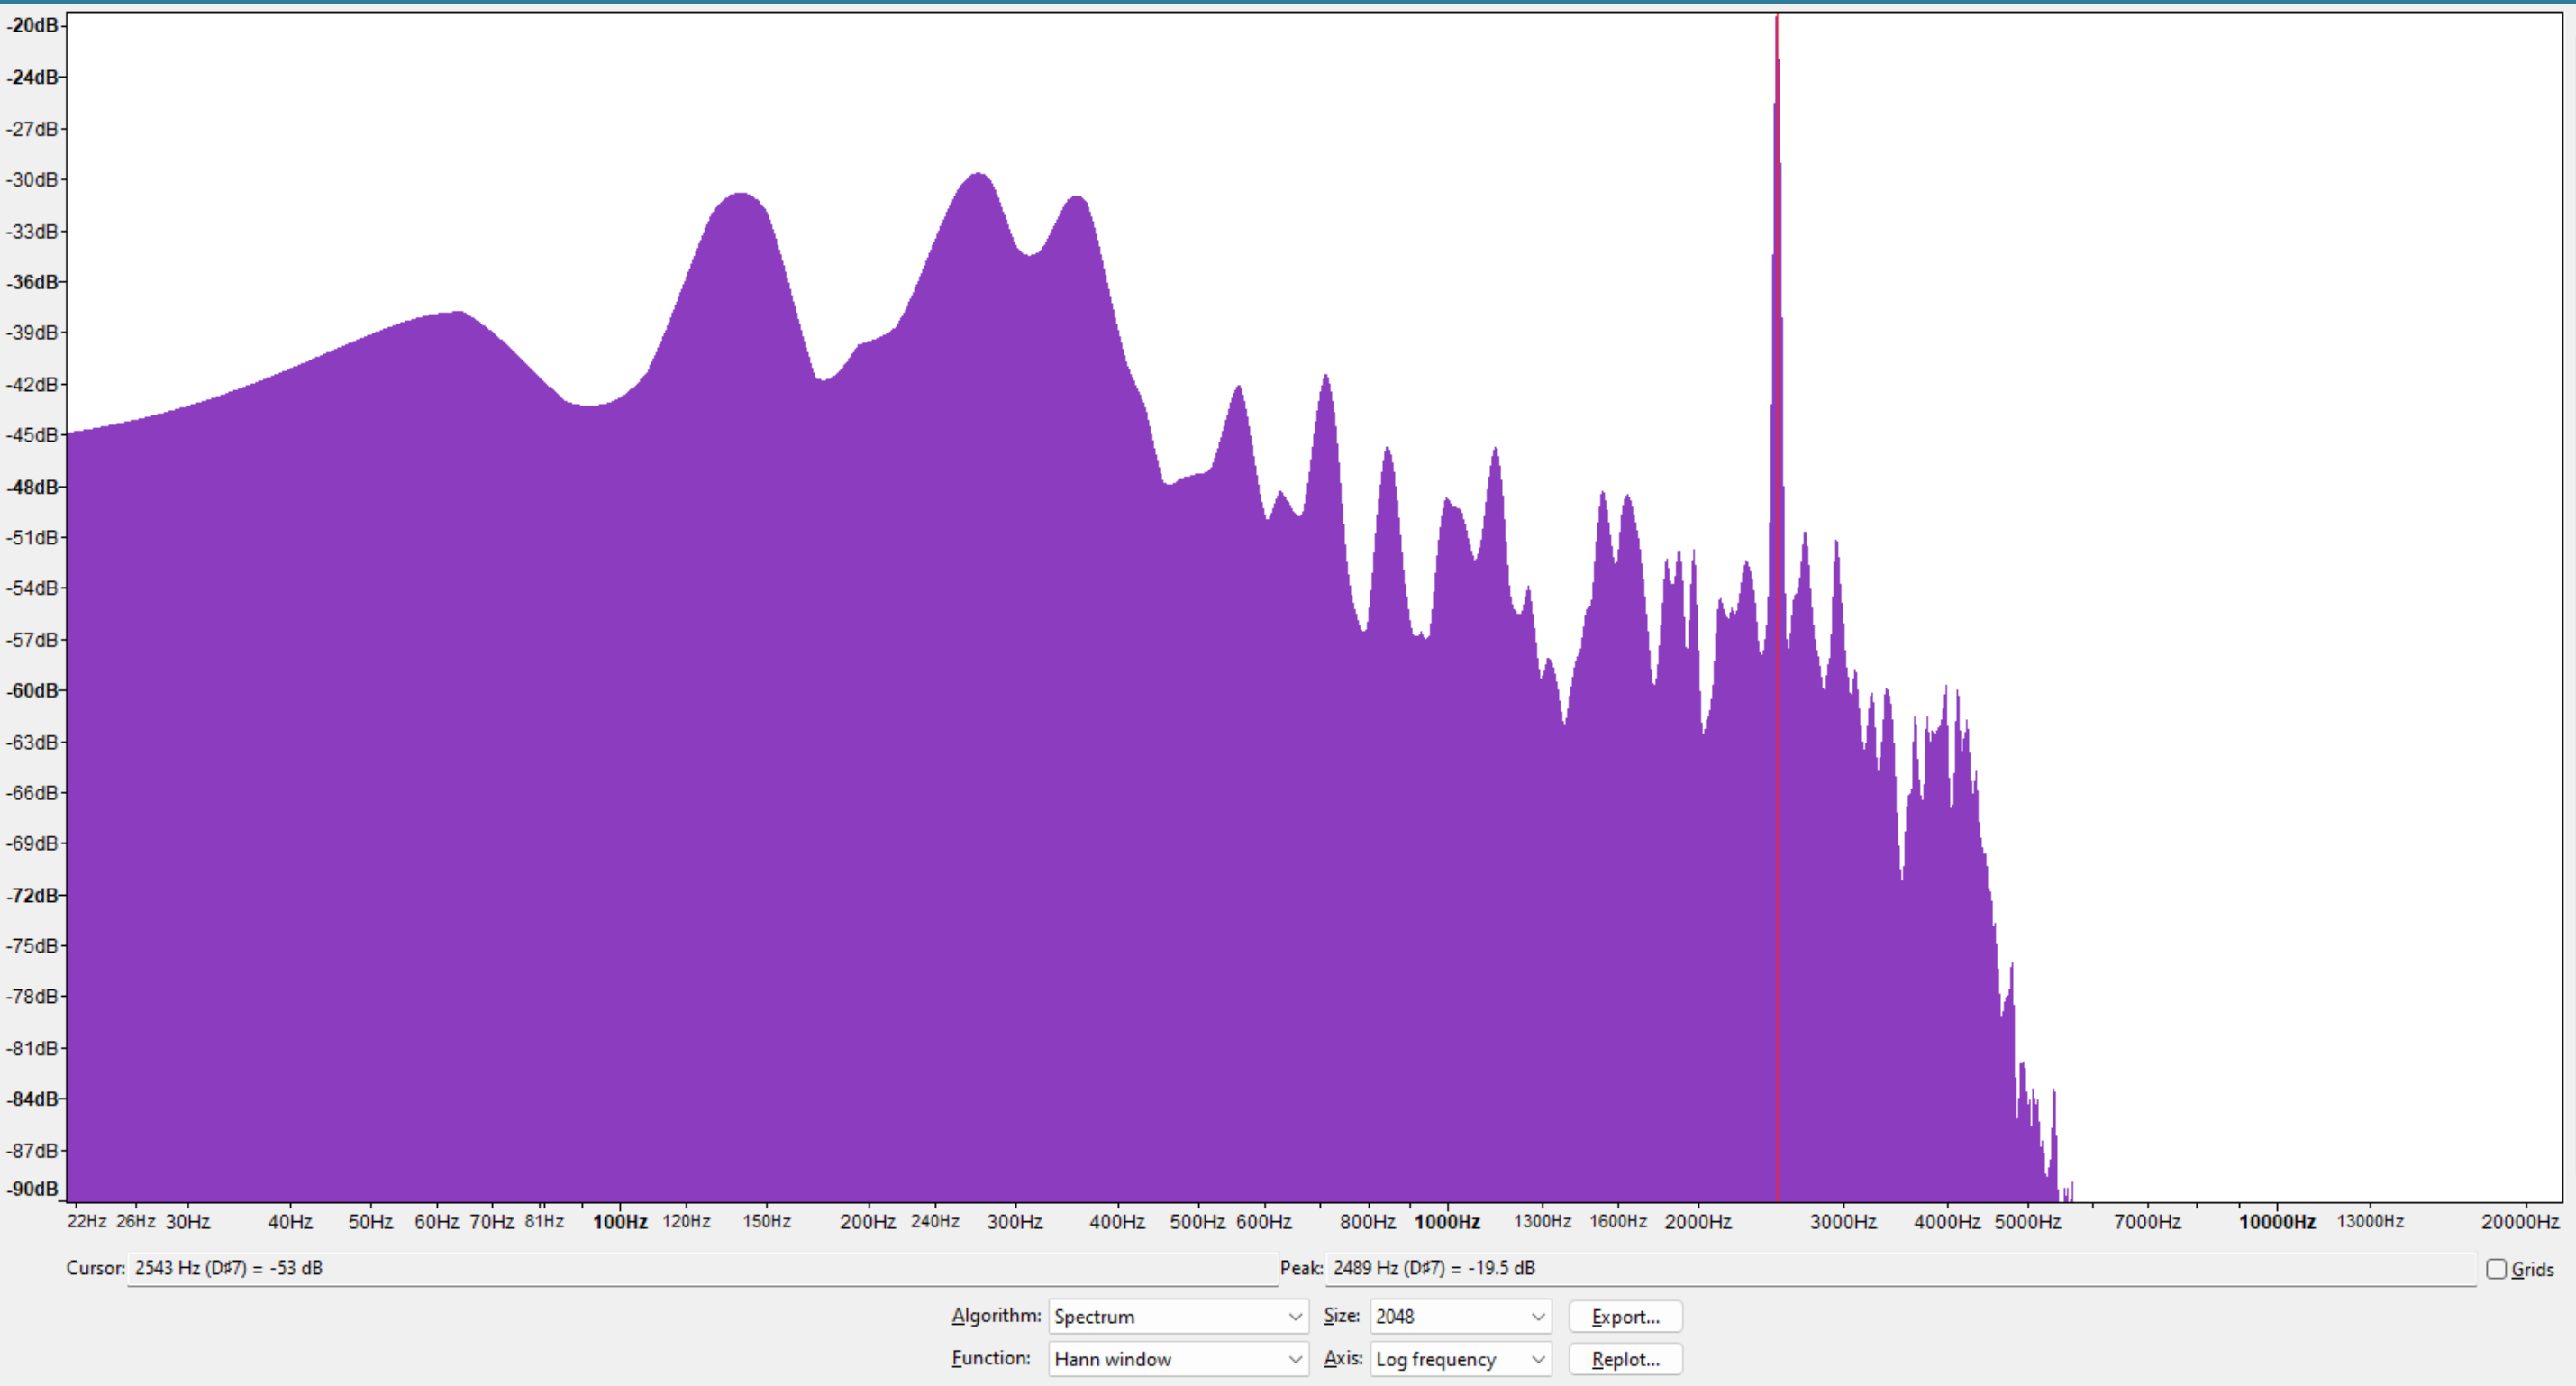
\includegraphics[width=1\textwidth]{Bilder/Audio_sectrum.png}
	\caption{Frekvensanalyse med Audacity}
	\label{fig:fig3}
\end{figure}

Med utgangspunkt i hvilke komponenter som er tilgjengelig så er store deler av filteret allerede bestemt. Spolen som ble brukt var på $101.9mH$ som ble målt og verifisert i tidligere arbeid. Motstanden settes til $1k\Omega$ i begynnelsen av testingen ettersom den kun skalerer spenningen ut av filteret og er defor ikke med på å bestemme frekvensen til filteret. For å beregne verdien til kondensatoren så tar man utgangspunkt i formelen for resonansfrekvensen til et RLC filter \ref{eq:1} og løser det med hensyn på kondensatoren \ref{eq:2}. Kondensatoren blir da $C = 40nF$ siden den kan lett lages ved å paralellkoble 4 kondensatorer på $10nF$ hver.

\begin{equation}
	f_0 = \frac{1}{2\pi \sqrt{LC}}
	\label{eq:1}
\end{equation}


\begin{equation}
	C = \frac{1}{(2\pi f_0)^2 L}
	\label{eq:2}
\end{equation}

\begin{equation}
	C = \frac{1}{(2\pi \cdot 2489Hz)^2 \cdot 101.9mH} = 4.01645 \cdot 10^-8 \approx 40nF
	\label{eq:3}
\end{equation}

For å verifisere at filteret fungerer som det skal så ble det simulert i \href{https://www.falstad.com/afilter/circuitjs.html?cct=$+1+0.000005+5+50+5+40%0A%25+0+28853.998118144256%0Al+912+208+912+304+0+0.1018+0%0Ac+912+304+912+400+0+4e-8+0%0Ar+800+208+912+208+0+1000%0AO+912+208+976+208+0%0Ag+912+400+912+432+0%0A170+800+208+768+208+3+20+60+5+0.5%0Ao+5+64+0+34+5+0.00009765625+0+-1+in%0Ao+3+64+0+34+5+0.00009765625+1+-1+out%0Ao+0+64+0+34+10+0.025+2+-1+inductor%0Ao+1+64+0+34+10+0.025+2+-1+cap%0A}{Falstad} og det ble laget et bilde av simuleringen som er vist i figur \ref{fig:fig4}.

\begin{figure}[!h]
	\centering
	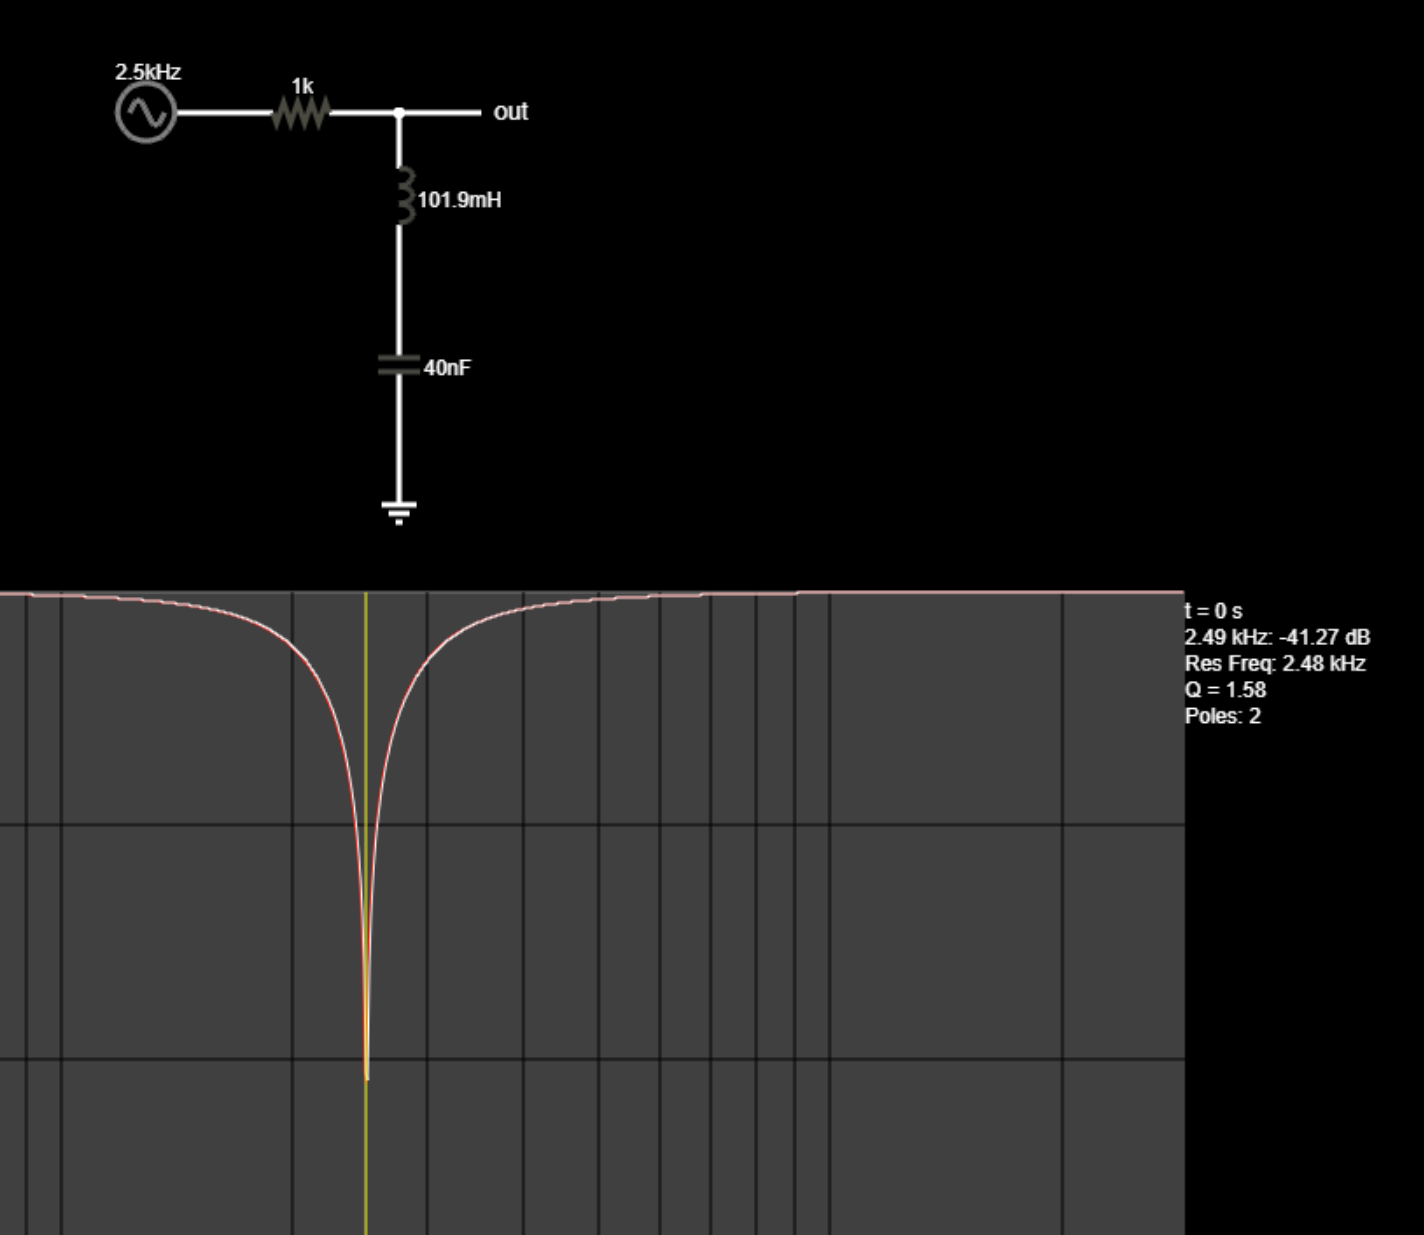
\includegraphics[width=0.8\textwidth]{Bilder/Falstad_filters.png}
	\caption{Simulert filter i Falstad}
	\label{fig:fig4}
\end{figure}


For å teste filteret ble Analog Discovery 2 brukt for å genere lydsignalet og måle spenningen på utgangen av filteret. For å sørge for at eventuelle hodetelefpner eller anndre systemer utenfor kretsen skal påvirke systemet blir det lagt til en op-amp for å buffre signalet. I figur \ref{fig:fig5} er det vist et bilde av hvordan filteret ble koblet opp.

\begin{figure}[!h]
	\centering
	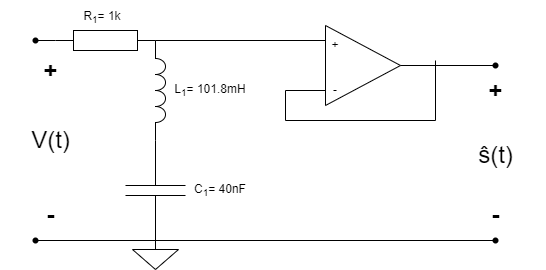
\includegraphics[width=0.7\textwidth]{Bilder/RLC_filter.drawio.png}
	\caption{Kobling av filteret}
	\label{fig:fig5}
\end{figure}


Først ble filteret testet ved å kjøre en netverksanalyse på det og generere et bodeplot av dataen i python. I figur \ref{fig:fig6} er det vist et bodeplot av filteret. Det er tydelig at filteret har mest demping på 2460Hz men det er også 23 dB demping på 2489Hz. 

\begin{figure}[!h]
	\centering
	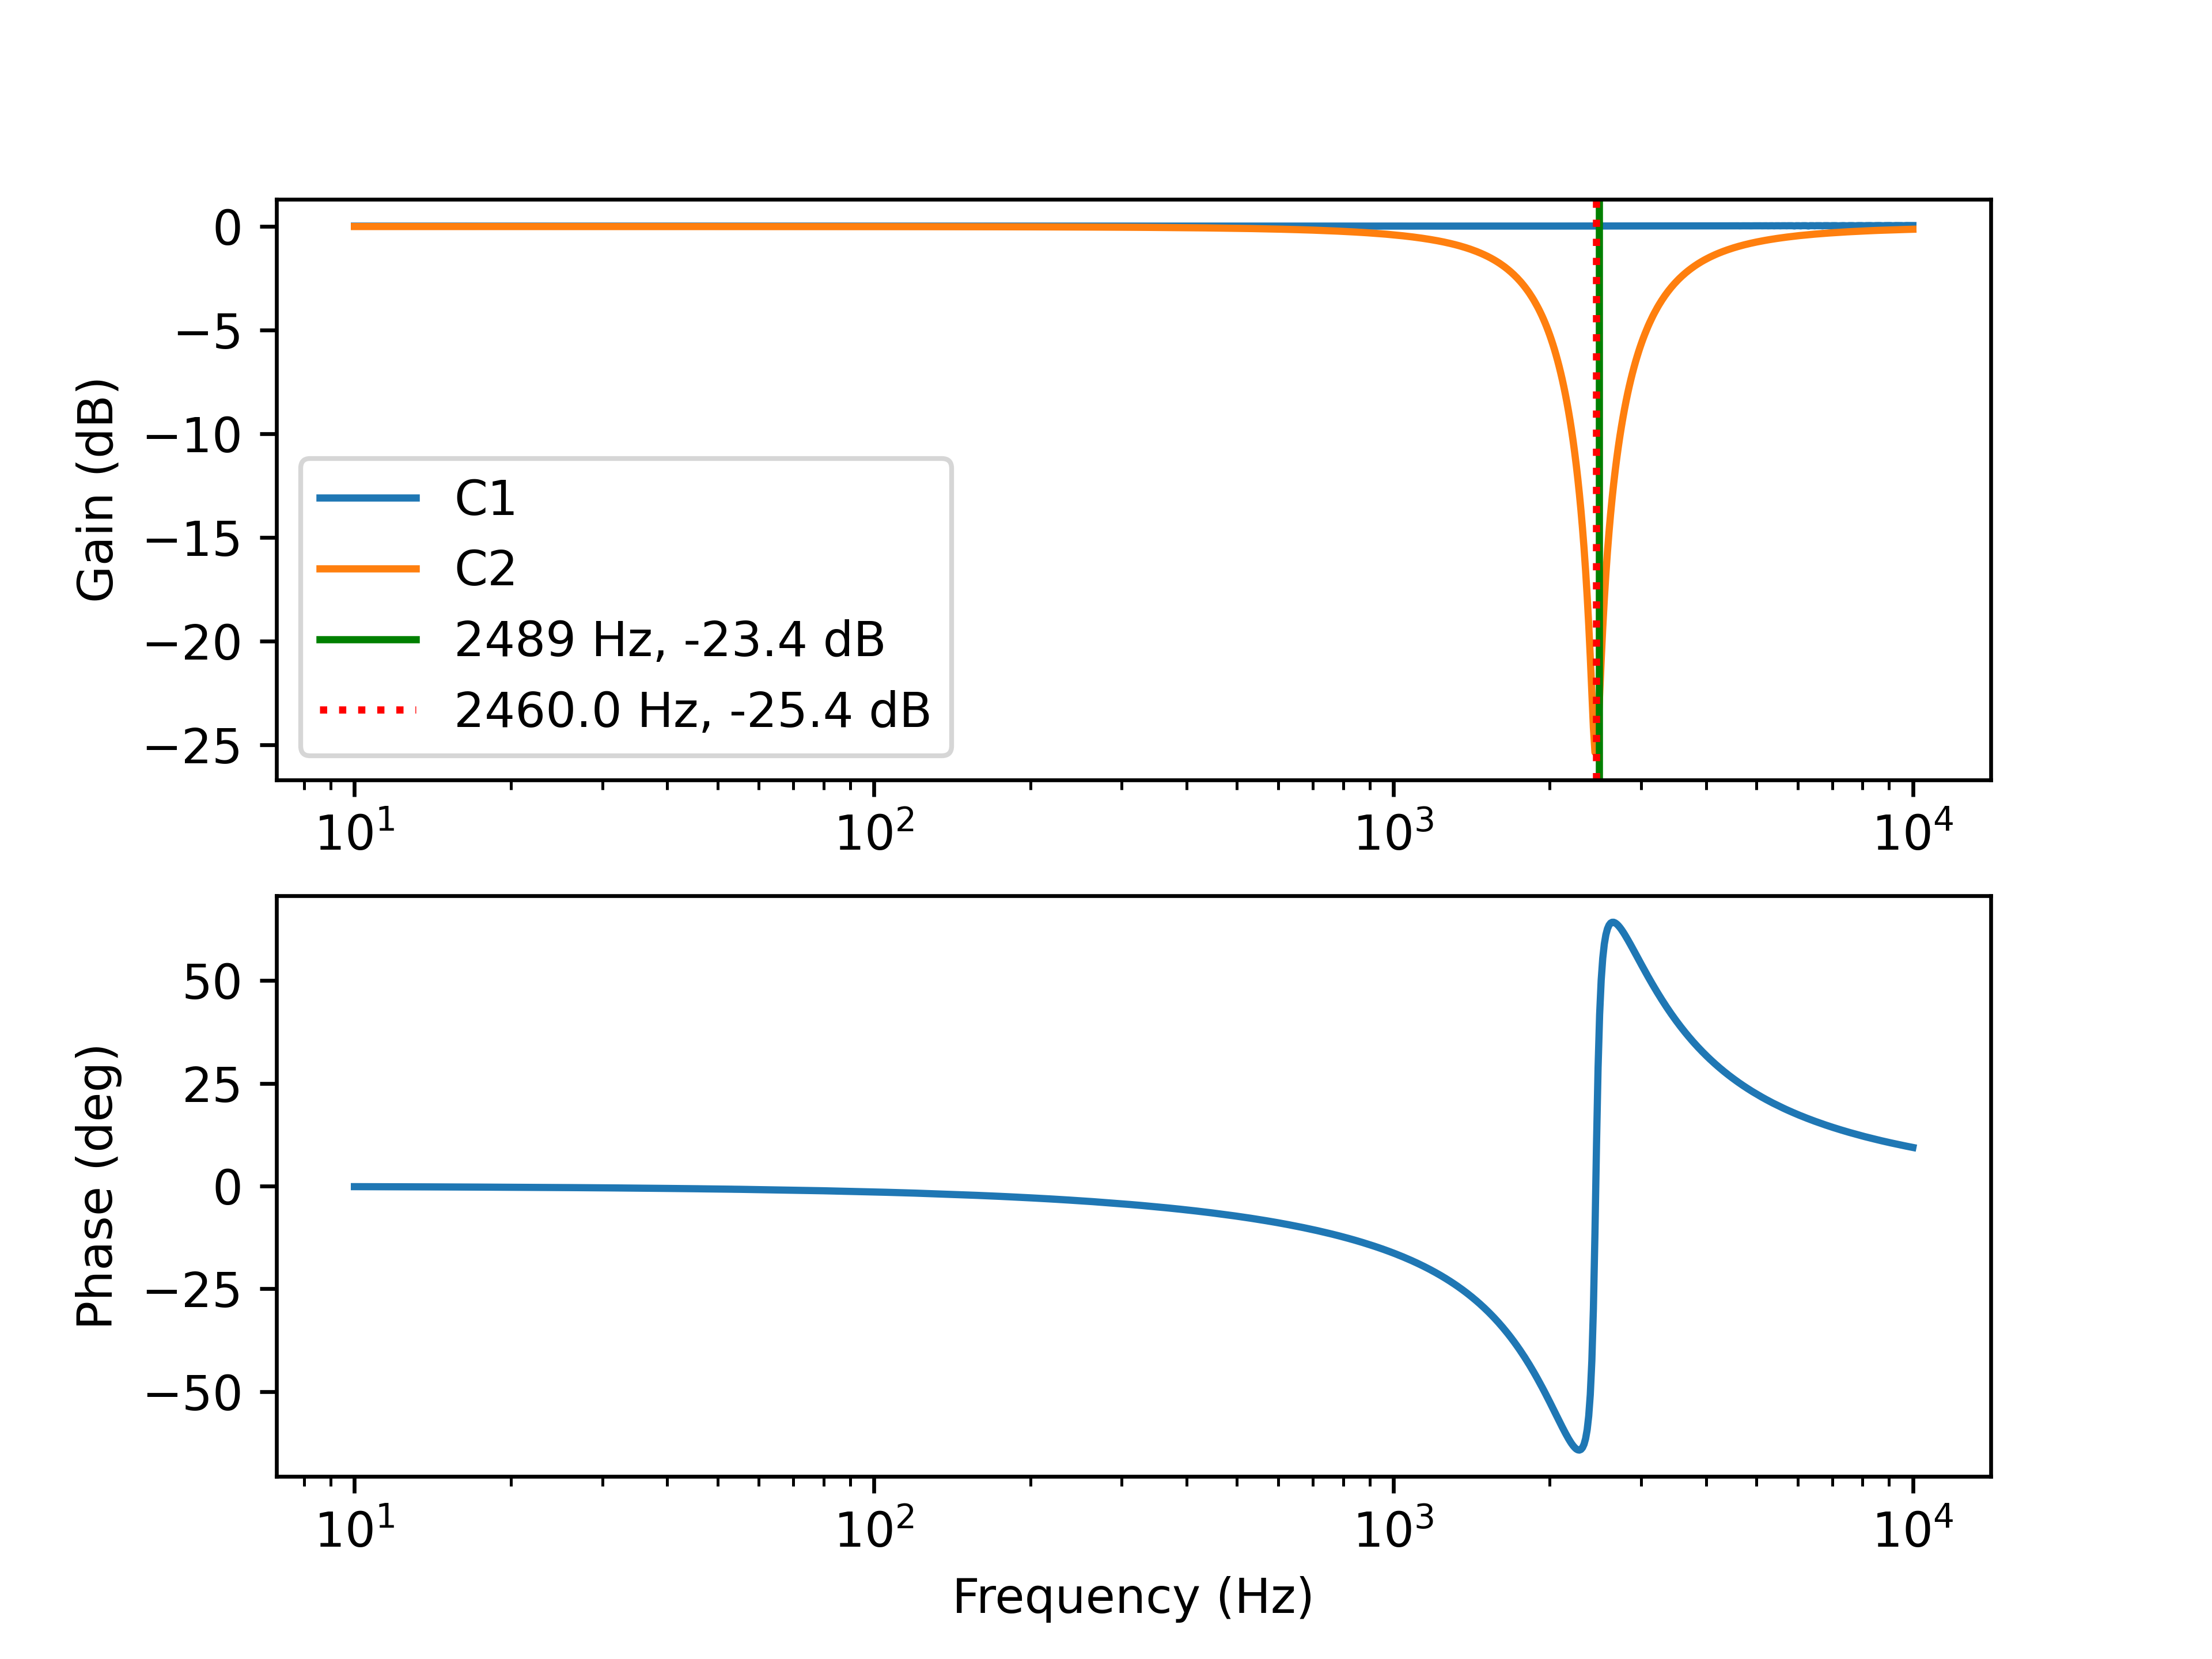
\includegraphics[width=1\textwidth]{Bilder/bode1K.png}
	\caption{Bodeplot av filteret}
	\label{fig:fig6}
\end{figure}

For å teste hvorvit realiseringen faktisk fungerer så ble ble lydfilen spilt gjennom filteret og en spektrumsanalyse ble gjort på utgangssignalet til filteret med WaveForms. Pipelyden er tydelig redusert i lydklippet og med spektrumsanalysen i figur \ref{fig:fig7} er det tydelig at pipelyden er redusert med 24.5dB. 

\begin{figure}[!h]
	\centering
	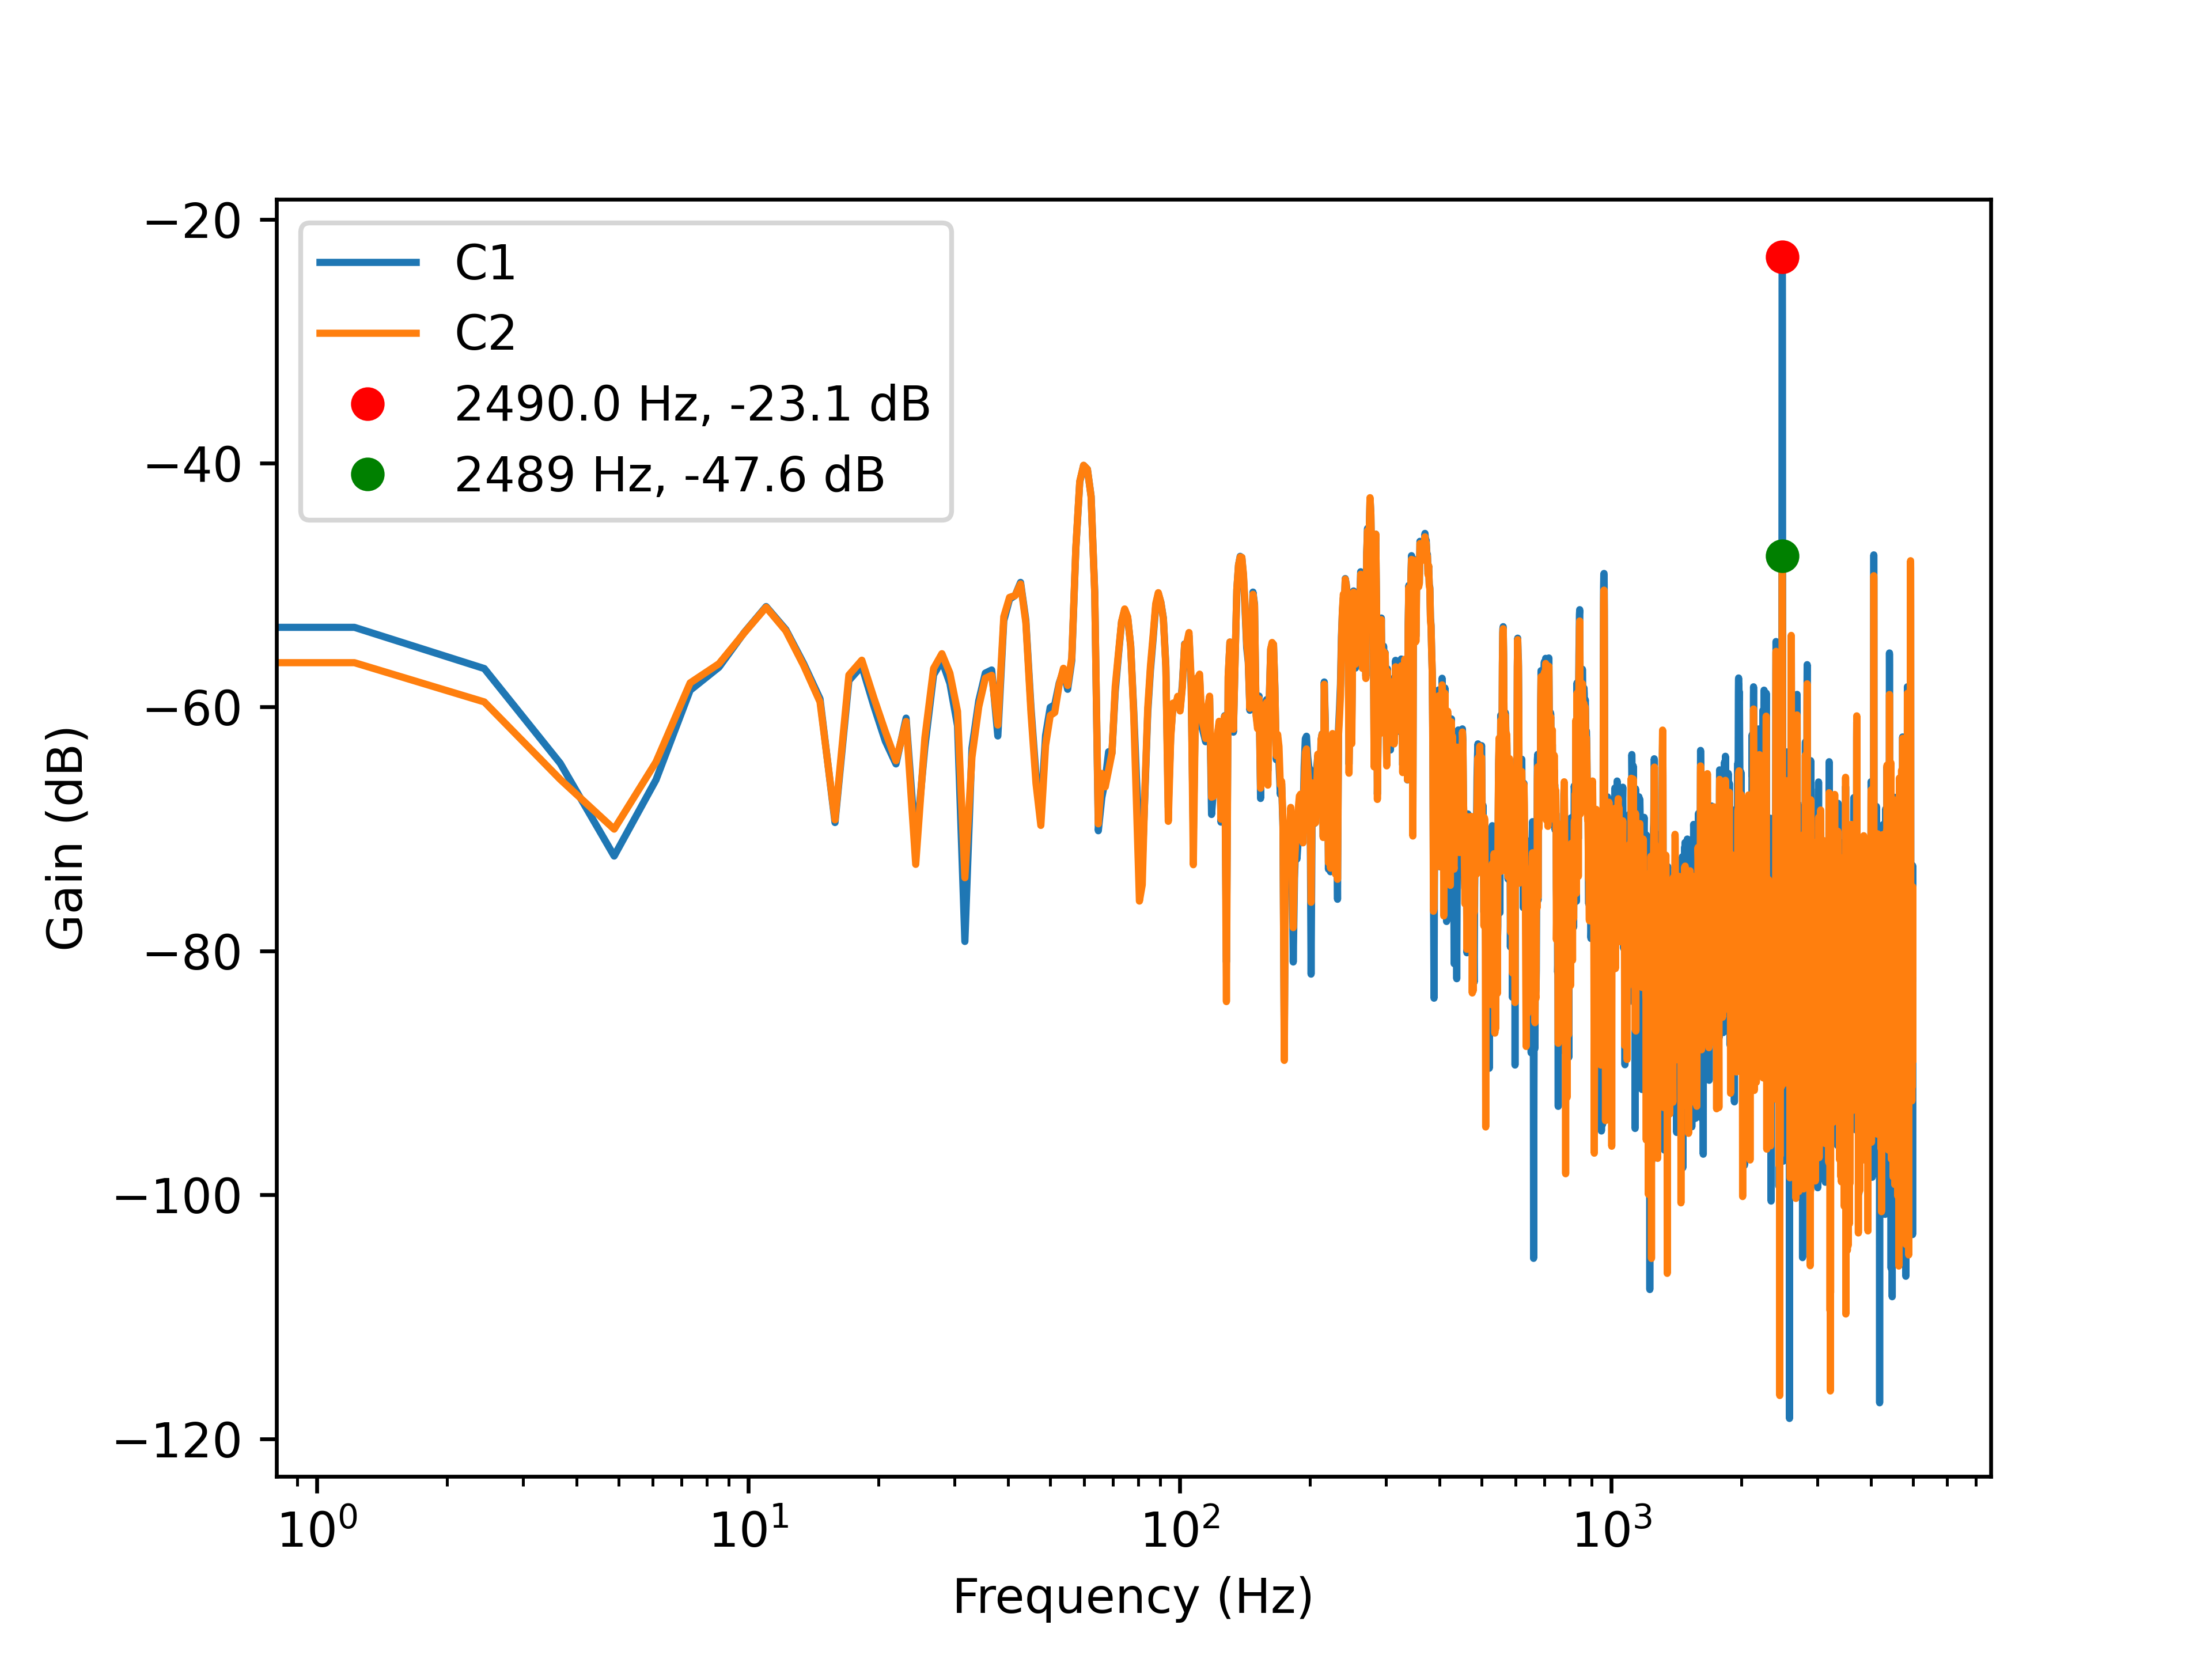
\includegraphics[width=1\textwidth]{Bilder/spectrum2K.png}
	\caption{Spektrumsanalyse av filteret}
	\label{fig:fig7}
\end{figure}

Problemstillingen var å forbedre signalkvaliteten til en lydfil, men siden pipetonen fremdeles kan høres så anses det derfor som en delvis løsning. For å få en fulstendig løsning så blir det konstruert et identisk filter i serie med det første filteret. Dette filteret vil ha samme resonansfrekvens, men grunnet unøyaktige komponenter så må det utregnes en ny kondensatorverdi med formelen i \ref{eq:2}. Den nye spolen har en verdi på $91.8mH$. Den optimale kondensatorverdien blir da $44.5nF$ som sett i utregning \ref{eq:4}, men kondensatoren blir realisert med $C = 44.7nF$ som er vist i figur \ref{fig:fig8}.

\begin{equation}
	C = \frac{1}{(2\pi \cdot 2489Hz)^2 \cdot 91.8mH} = 4.45398 \cdot 10^-8 \approx 44.5nF
	\label{eq:4}
\end{equation}

\begin{figure}[!h]
	\centering
	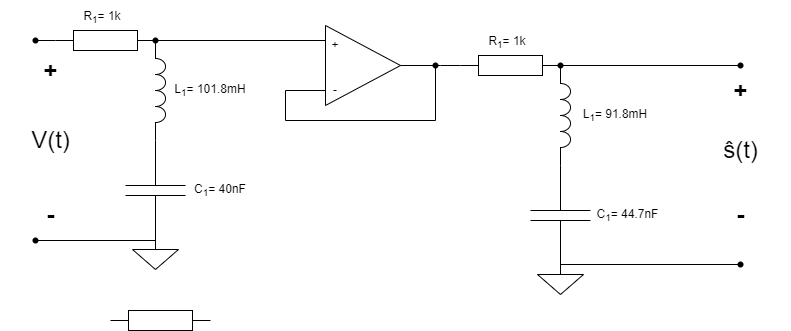
\includegraphics[width=0.8\textwidth]{Bilder/RLC_filterV2.drawio.png}
	\caption{Design nummer to}
	\label{fig:fig8}
\end{figure}

Når det blir gjort identiske tester kan man se tydelig forbedring i lydklippet, og det pipelyden er ikke lenger hørbar. I bodeplottet, \ref{fig:fig9}, og i spektrumsanalysen, \ref{fig:fig10} kan det leses ut en ny dempning på $40.8dB$.

\begin{figure}[!h]
	\centering
	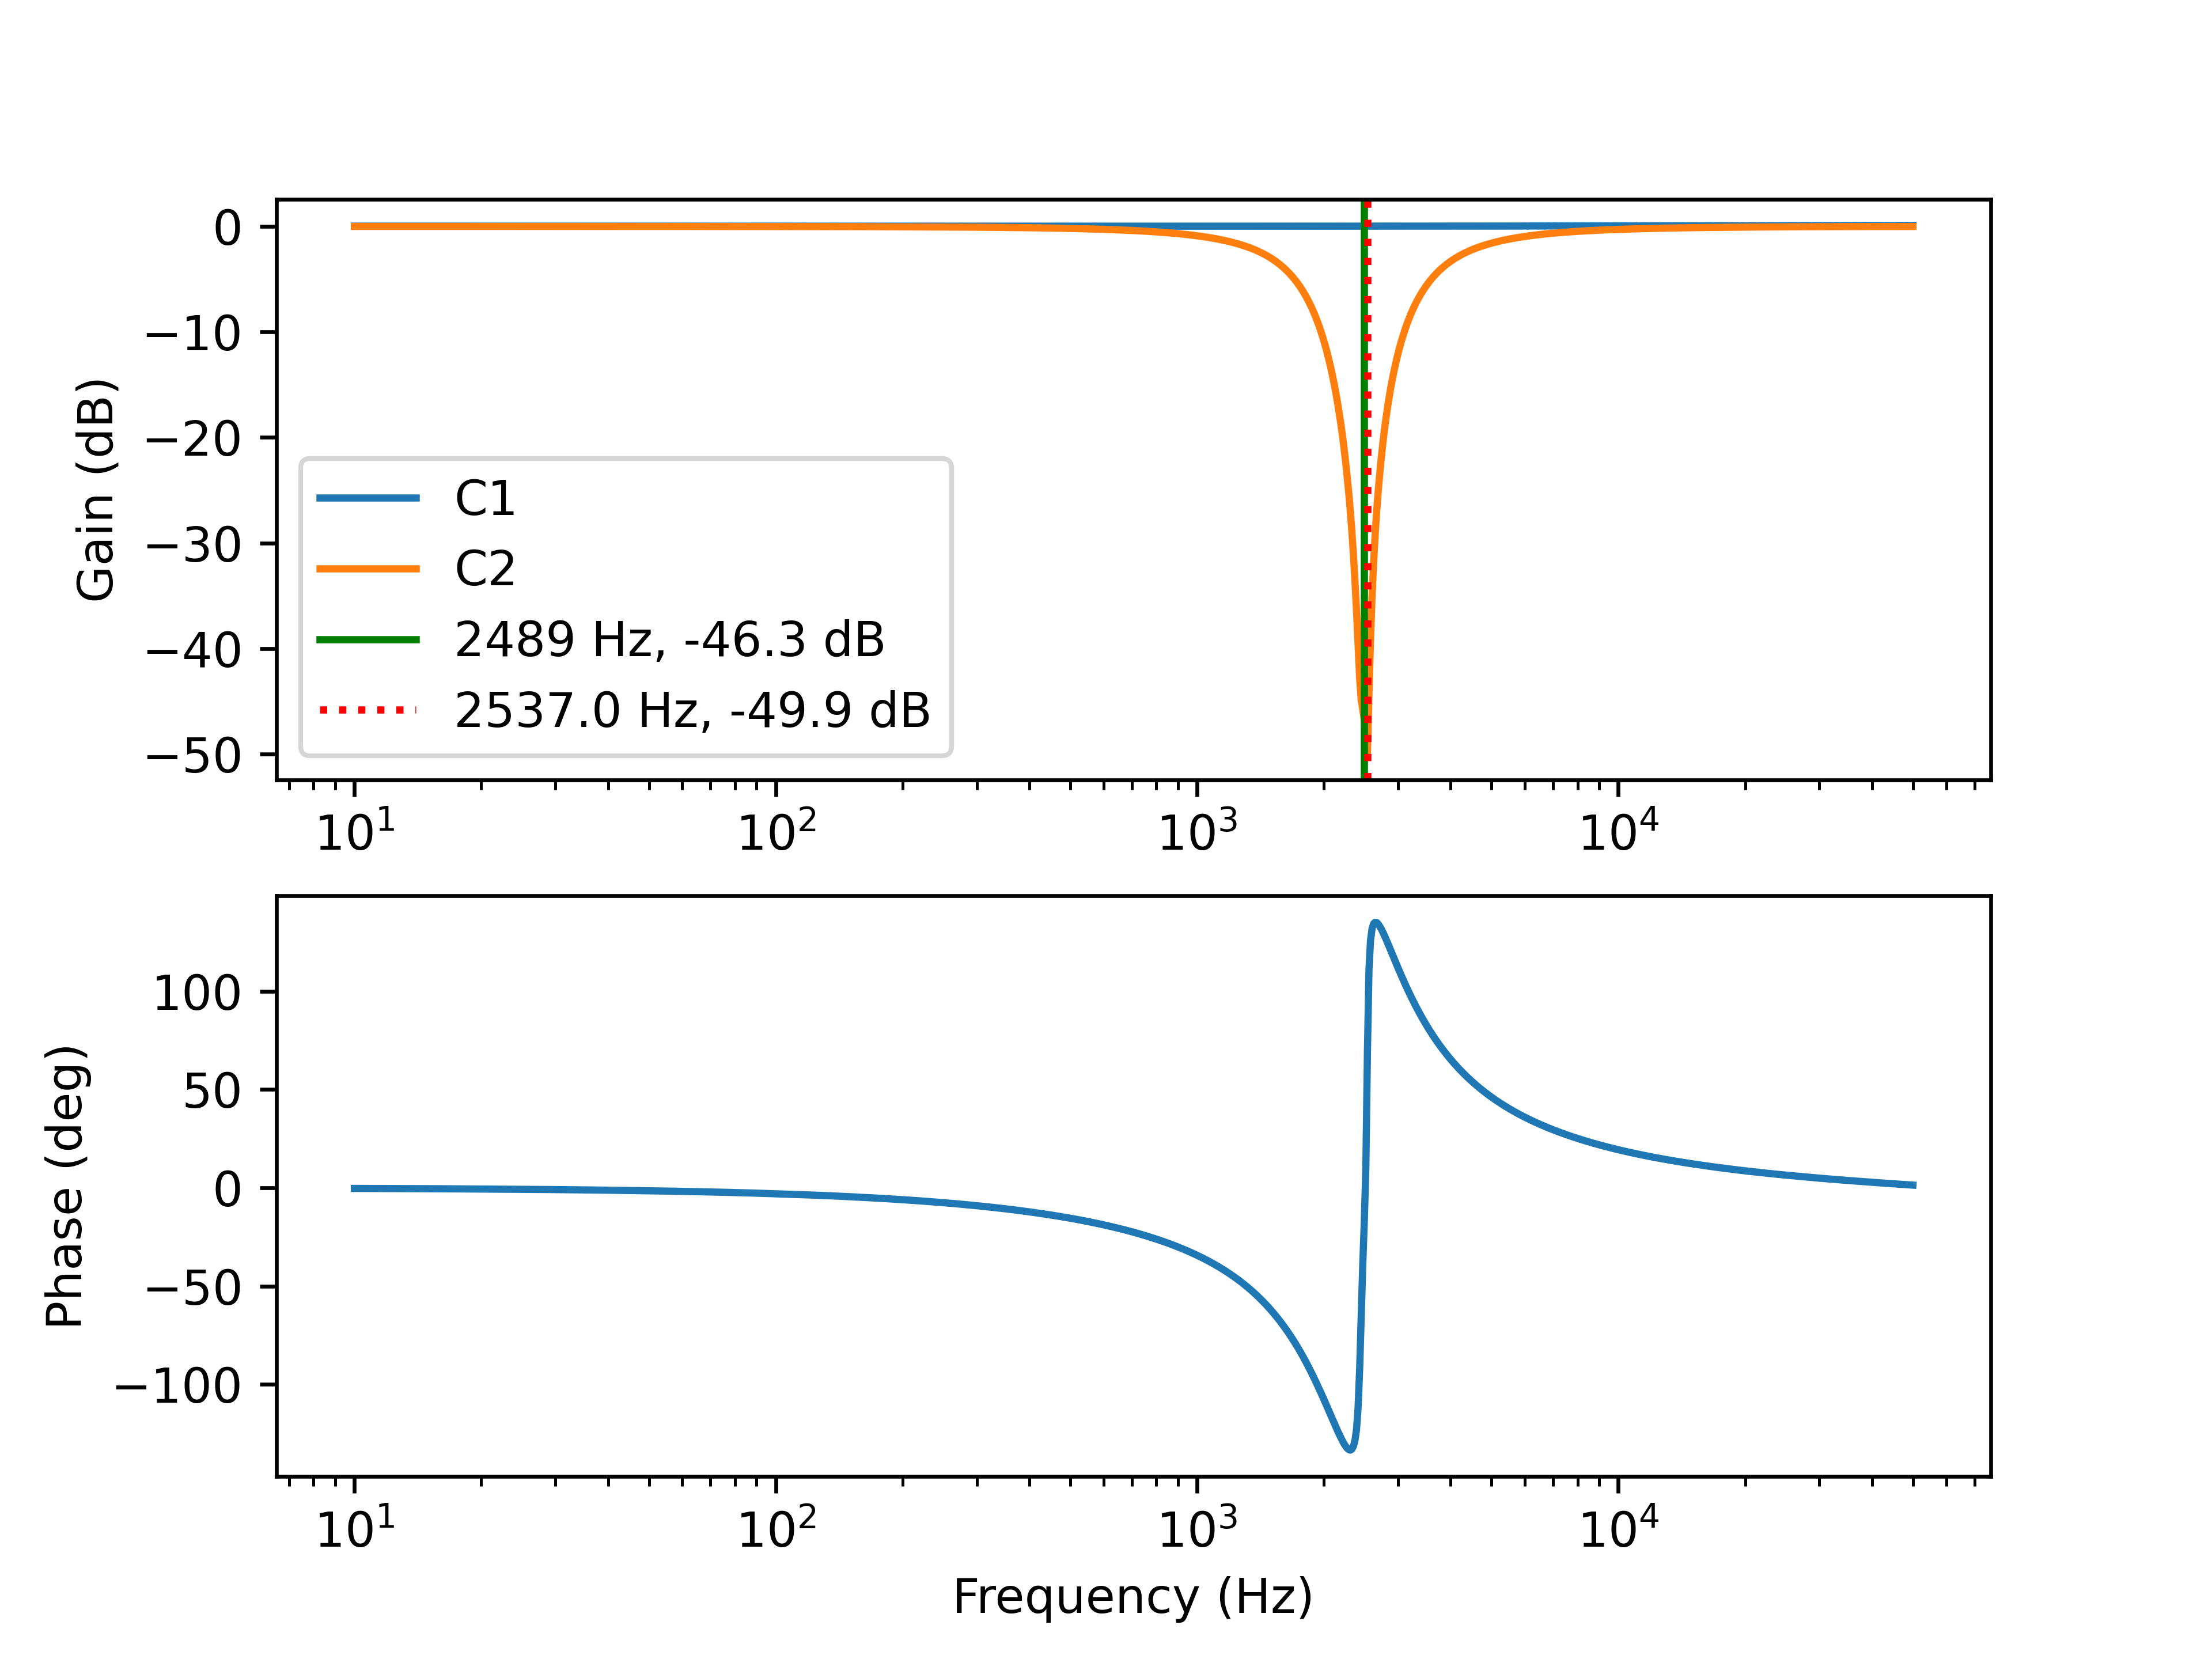
\includegraphics[width=0.8\textwidth]{Bilder/bode2x1K.png}
	\caption{Bodeplot av filteret}
	\label{fig:fig9}
\end{figure}

\begin{figure}[!h]
	\centering
	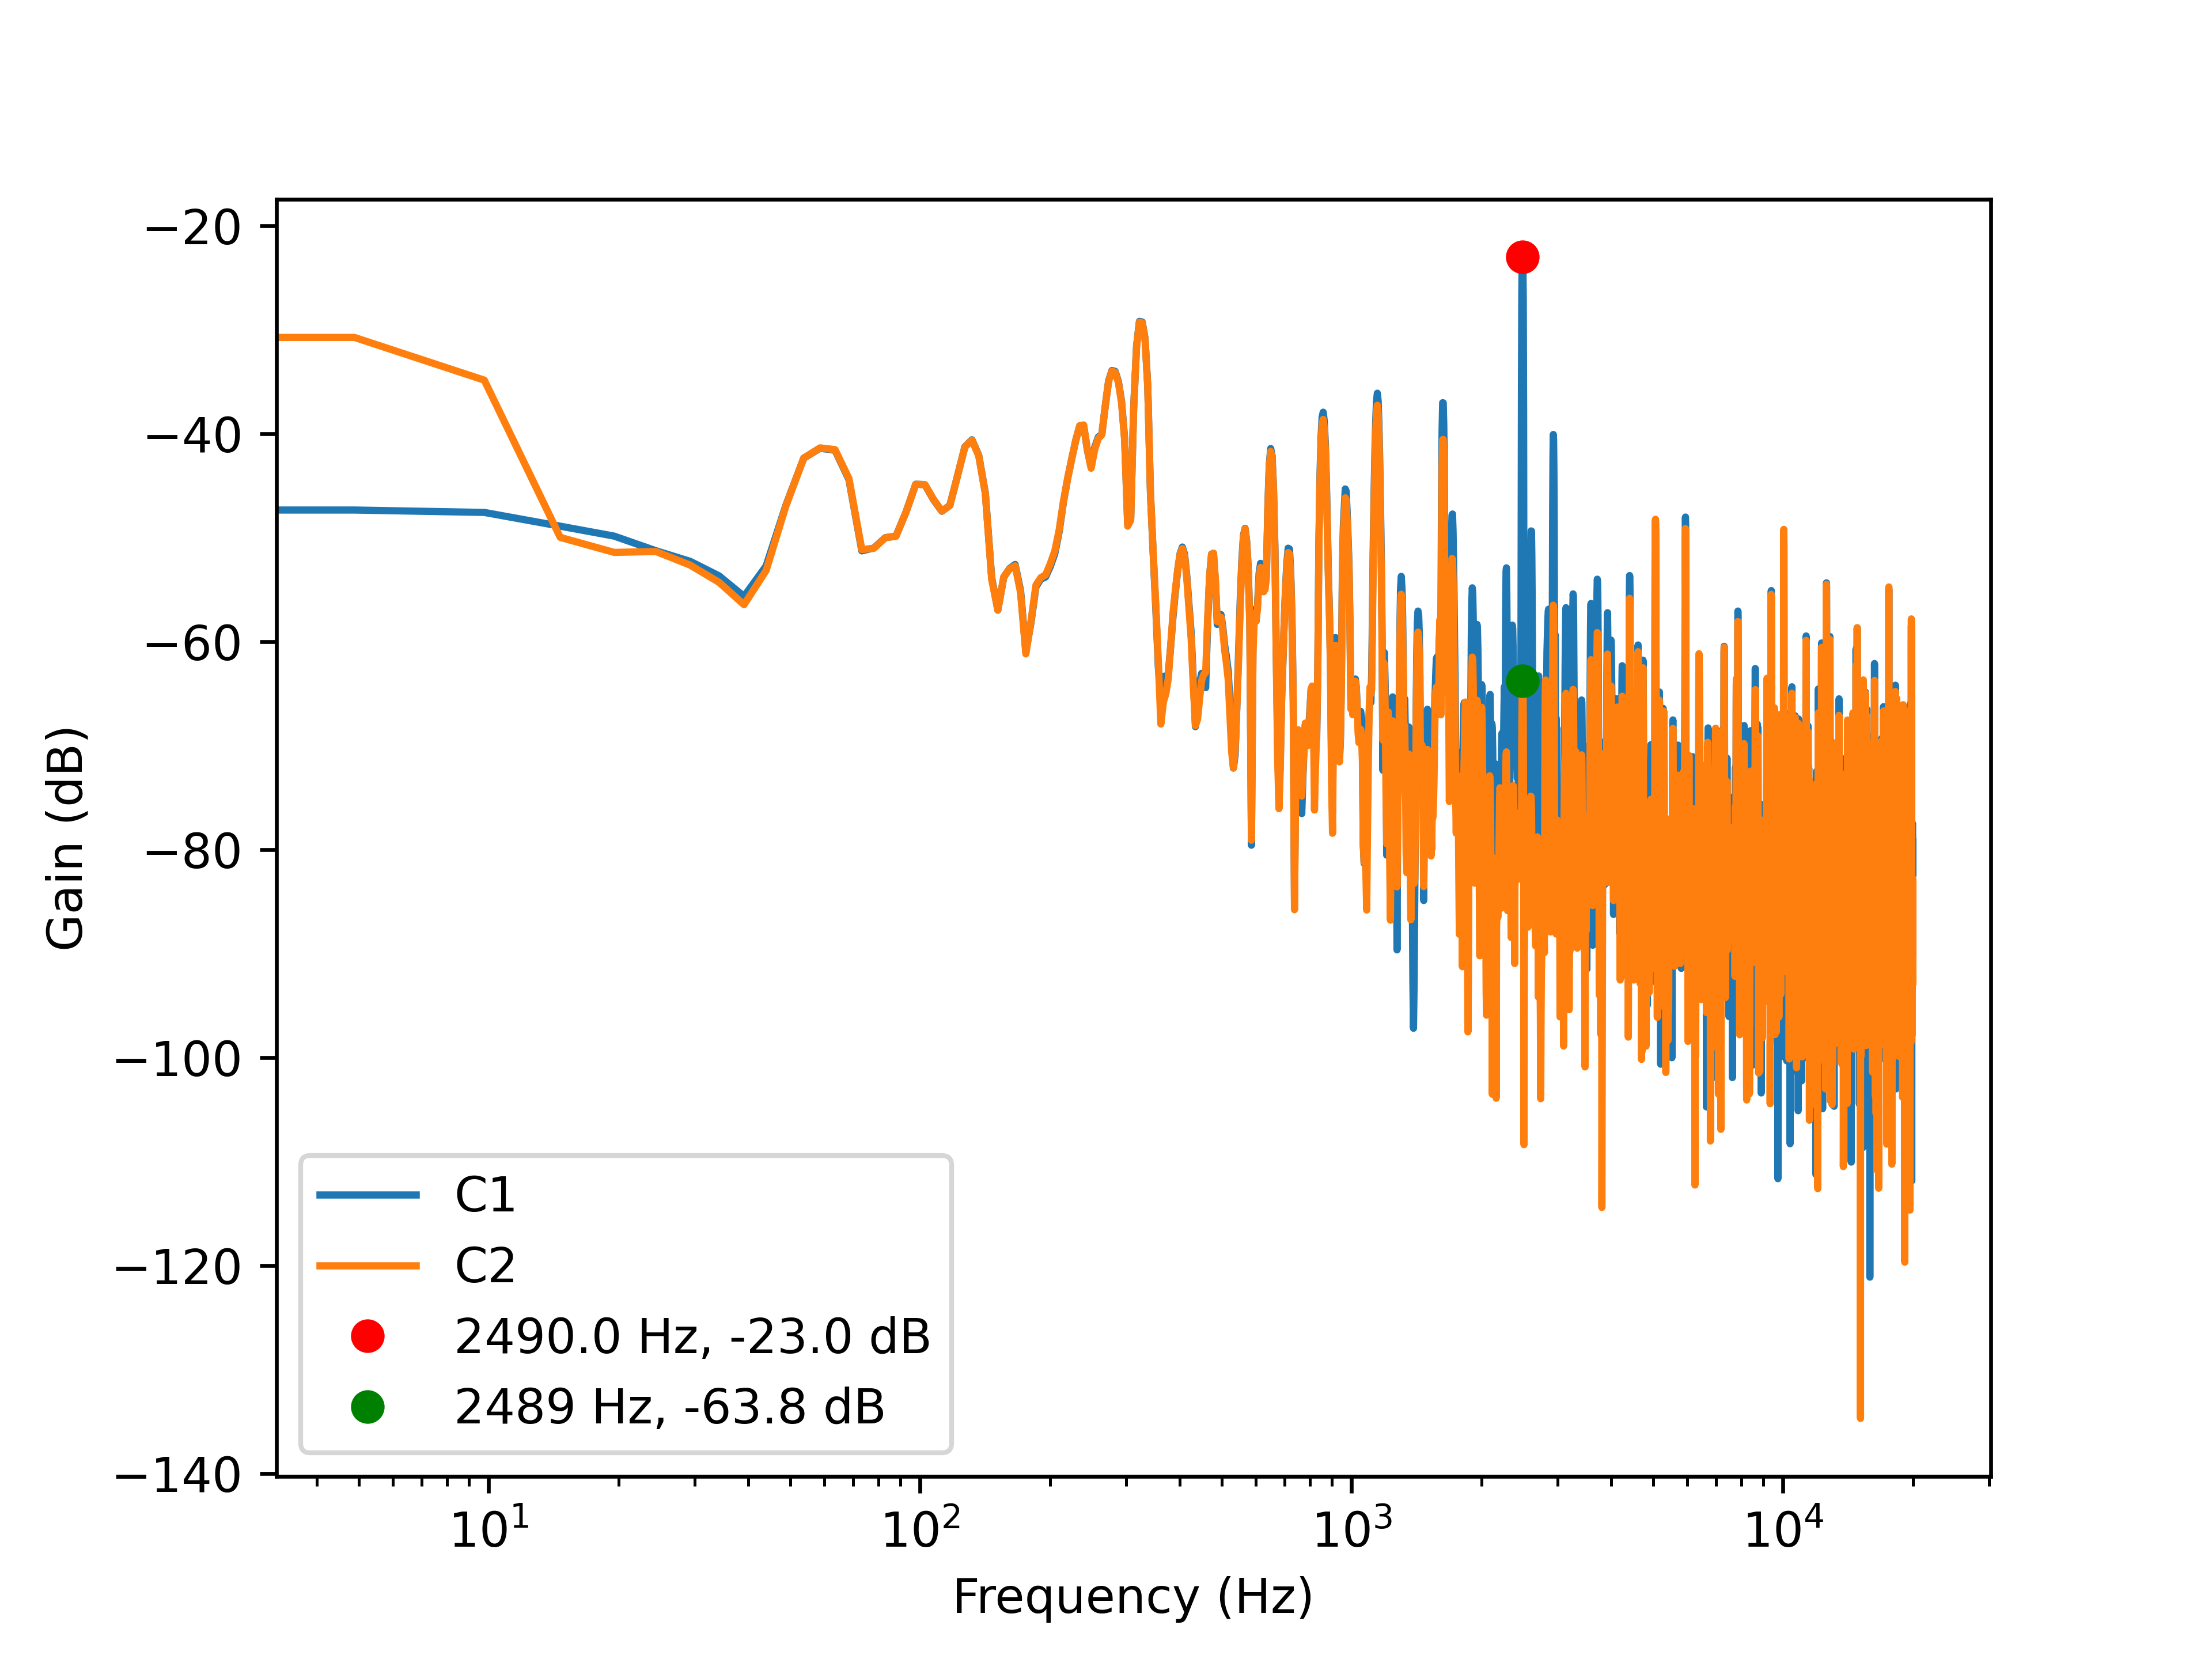
\includegraphics[width=0.8\textwidth]{Bilder/spectrum2x1K.png}
	\caption{Spektrumsanalyse av filteret}
	\label{fig:fig10}
\end{figure}
